\documentclass{article}

\usepackage{amsmath,amssymb}
\usepackage{fullpage}
\usepackage{enumerate}
\usepackage{hyperref}
\usepackage{tikz,tkz-euclide}
\usepackage{float}

\begin{document}

\begin{center}
\textbf{\Large Senior February Monthly Problem Set}
\\ \vspace{1em}
\textbf{\large Solutions}
\end{center}

\begin{enumerate}[1.]

\item % SW-2013-3
{\itshape Let $n$ be a positive integer. Both $n$ and $n^2$ only contain the digits $1$, $2$ and $3$ (not necessarily all of them). Determine all possible values of $n$.}

If $n \equiv 2 \text{ or } 3 \pmod{10}$, then we have that $n^2 \equiv 4 \text{ or } 9 \pmod{10}$, and so $n$ is not a solution. We thus require that $n \equiv 1 \pmod{10}$.

If $n > 10$, then we have that $n \equiv 11 \text{ or } 21 \text{ or } 31 \pmod{100}$. If $n \equiv 21 \pmod{100}$, then $n^2 \equiv 41 \pmod{100}$, and so $n$ is not a solution. Similarly, if $n \equiv 31 \pmod{100}$, then $n^2 \equiv 61 \pmod{100}$, and so $n$ is not a solution. We thus require that $n \equiv 11 \pmod{100}$.

If $n > 100$, then $n \equiv 111 \text{ or } 211 \text{ or } 311 \pmod{1000}$. If $n \equiv 211 \pmod{1000}$, then we have that $n^2 \equiv 521 \pmod{1000}$, and so $n$ is not a solution. Similarly, if $n \equiv 321 \pmod{1000}$, then $n^2 \equiv 41 \pmod{1000}$, and so $n$ is not a solution. We thus require that $n \equiv 111 \pmod{1000}$.

Finally, if $n > 1000$, then we must have that $n \equiv 1111 \text{ or } 2111 \text{ or } 3111 \pmod{10000}$. If $n \equiv 1111 \pmod{10000}$, then we have that $n^2 \equiv 4321 \pmod{10000}$, and so $n$ is not a solution. If $n \equiv 2111 \pmod{10000}$, then $n^2 \equiv 6321 \pmod{10000}$, and if $n \equiv 3111 \pmod{10000}$, then $n^2 \equiv 8321 \pmod{10000}$. In each case we find that $n$ is not a solution.

We see that the only possible values for $n$ are $1$, $11$, and $111$.


\vspace{6pt}
\item % DB-2012-2
{\itshape Given a (not necessarily convex) quadrilateral $ABCD$, call a point $P$ in the same plane as $ABCD$ an \emph{areal centre} for $ABCD$, if any line through $P$ divides $ABCD$ into two parts of equal area. What are necessary and sufficient conditions on $ABCD$ for it to possess an areal centre?}


\vspace{6pt}
\item % The Liam
{\itshape The (English language version of the) game of Scrabble\texttrademark{} consists of 100 tiles, each containing either a letter from A to Z (some letters occur more than once), except for two blank tiles; see \href{https://en.wikipedia.org/wiki/Scrabble_letter_distributions#English}{\texttt{the relevant Wikipedia page}} for the exact distribution of multiplicities of each letter.

In a solo game of Scrabble, the player starts by choosing seven tiles from the 100 available tiles at random. What is the probability that the player does not pick up any vowels?}


\vspace{6pt}
\item % The Robin
{\itshape For each pair of positive integers $(a, b)$, prove that there exists infinitely many positive integers $n$ such that
\[ \frac{a^n + 1}{n^b + 1} \]
is not an integer.}

We will show that there are infinitely many integers $n$ such that there is a prime $p$ such that $p \mid n^b + 1$ but $p \nmid a^n + 1$.

We note that for any prime $p$, there exists a natural number $n$ such that $p \mid n^b + 1$ if and only if $-1$ is a $b^\text{th}$ power modulo $p$. It is sufficient that $2b \mid p - 1$, in which case we have that $g^{(p - 1)/2b}$ is a $b^\text{th}$ root of $-1$ modulo $p$, where $g$ is a primitive root modulo $p$.

Thus let $p$ be a prime such that $p \equiv 1 \pmod{2b}$ and note that for such a prime $p$ we have $p \neq 2$. (There are infinitely many such primes by Dirichlet's Theorem, but we only need one.)

If $p - 1 \mid n$, then we note that by Fermat's Little Theorem, we have $a^n \equiv 0 \text{ or } 1 \pmod p$, and so $a^n + 1 \equiv 1 \text{ or } 2 \pmod p$. In particular, since $p \neq 2$, we have that $p \nmid a^n + 1$. 

We are thus finished if there are infinitely many $n$ such that $p - 1 \mid n$, and $n \equiv g^{(p - 1)/2b} \pmod p$. Since $\gcd(p, p - 1) = 1$, there infinitely many such $n$ by the Chinese Remainder Theorem.

\vspace{6pt}
\item % DB-2012-9
{\itshape Call a positive integer a \emph{triangular} number if it is of the form $1 +2 +3 +\dotsb +k$ for some positive integer k, and \emph{pentagonal} if it is of the form $1 +4 +7 +10 +13 +\dotsb +(3n-2)$ for some positive integer $n$. Prove that there are infinitely many cases where the product of two consecutive pentagonal numbers is equal to the product of two consecutive triangular numbers.}

Using the formula for the sum of the terms in an arithmetic progression, one finds that the $k^\text{th}$ triangular number is given by
\[
	\frac{k(k + 1)}{2}
\]
and the $m^\text{th}$ pentagonal number is given by
\[
	\frac{m(3m - 1)}{2}.
\]

We thus wish to show that there are infinitely many $k$ and $m$ such that
\[
	\frac{k(k + 1)}{2} \cdot \frac{(k + 1)(k + 2)}{2} = \frac{m(3m - 1)}{2} \cdot \frac{(m + 1)(3m + 2)}{2},
\]
or equivalently such that
\[
	(k^2 + 2k + 1)(k^2 + 2k) = (3m^2 + 2m)(3m^2 + 2m - 1).
\]

We see that it is sufficient to show that there are infinitely many $k$ and $m$ such that $k^2 + 2k + 1 = 3m^2 + 2m$, or equivalently such that ${(3m + 1)}^2 - 3{(k + 1)}^2 = 1$.

We thus wish to show that the Pell equation $x^2 - 3y^2 = 1$ has infinitely many solutions where $x \equiv 1 \pmod 3$.

We note that one solution to the Pell equation is given by $x = 7$ and $y = 4$. Moreover, if $(x, y)$ is a solution such that $x \equiv 1 \pmod 3$, then $(7x + 12y, 4x + 7y)$ is another solution and satisfies $7x + 12y \equiv 1 \pmod 3$. There are thus infinitely many solutions such that $x \equiv 1 \pmod 3$, and we are done.

\vspace{6pt}
\item % Andrew
{\itshape Let $ABC$ be a triangle with circumcentre $O$. Let $D$ be the point of intersection between the bisector of $\angle ABC$ and the perpendicular bisector of $AB$. Let the circumcircle of $ADO$ be $\omega$. Let $E\neq A$ be the intersection of $\omega$ with the segment $AB$. Let $P\neq E$ be the intersection of the circumcircle of $COE$ with the line $AB$. Prove that $CP$ is tangent to $\omega$.}

\begin{figure}[H]
	\centering
	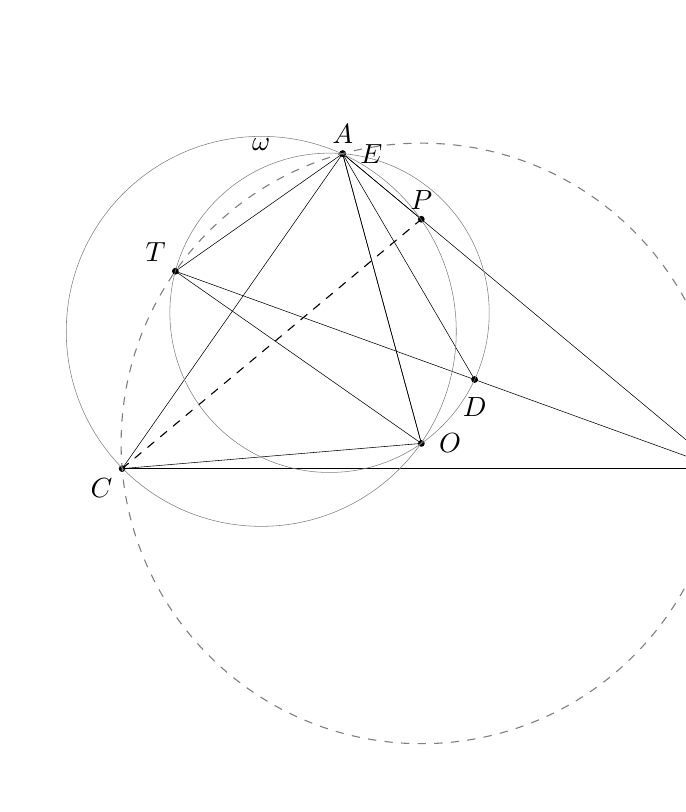
\begin{tikzpicture}[scale=4]
		\useasboundingbox (-1,-1) rectangle (1,1.4);
		\tkzDefPoints{0/1/A, 1.2/0/B, -0.7/0/C}
		\tkzDefCircle[circum](A,B,C)\tkzGetPoint{O}
		\tkzDefLine[bisector](A,B,C)\tkzGetPoint{b1}
		\tkzDefLine[mediator](A,B)\tkzGetPoints{m1}{m2}
		\tkzInterLL(B,b1)(m1,m2)\tkzGetPoint{D}
		\tkzDefCircle[circum](A,D,O)\tkzGetPoint{X}
		\tkzInterLC(A,B)(X,A)\tkzGetSecondPoint{E}
		\tkzDefCircle[circum](C,O,E)\tkzGetPoint{Y}
		\tkzInterCC(O,A)(X,A)\tkzGetFirstPoint{T}
		\tkzInterLC(A,B)(Y,C)\tkzGetFirstPoint{P}
		\tkzDrawPoints[fill=black](A,B,C,D,E,O,T,P)
		\tkzDrawSegments(A,B B,C C,A O,C O,T O,A O,E B,T D,A A,P A,T)
		\tkzDrawSegments[dashed,thin](C,P)
		\tkzDrawCircle(X,A)
		\tkzDrawCircle(Y,C)
		\tkzDrawCircle[dashed,thin](O,A)
		\tkzLabelPoints[below=0.1](D)
		\tkzLabelPoints[right=0.1](O,E)
		\tkzLabelPoints[above](A,P)
		\tkzLabelPoints[above left](T)
		\tkzLabelPoints[below left](B,C)
		\tkzLabelCircle[above=0.1](X,A)(30){$\omega$}
	\end{tikzpicture}
\end{figure}
Let $T$ be the midpoint of the arc $AC$ not containing $B$. We will show that $T$ lies on $\omega$. Note:
\begin{flalign*}
	\angle ADT&= \angle ABD + \angle DAB= 2\angle ABD=2\angle ABT=\angle AOT
\end{flalign*}
Therefore $T$ lies on $\omega$. Also note that since $\triangle OCT \equiv \triangle OAT$:
\begin{flalign*}
 	\angle CTO &= \angle TCO = \angle TAO
\end{flalign*}
So $CT$ is tangent to $\omega$. Let $P'= CT\cap AB$. We will show that $P' \equiv P$. Note that it is sufficient to show that $P'COE$ is a cyclic quad as this would require $P' \equiv P$. But note that:
\begin{flalign*}
 	\angle OEB= \angle OTA =\angle OAT=\angle OCT=\angle OCP
\end{flalign*}
So $P'COE$ is a cyclic quad, and so $P' \equiv P$ and thus $CP$ is tangent to $\omega$ at $T$.


\vspace{6pt}
\item % Dylan
{\itshape Call a function $f : \mathbb{N} \to \mathbb{N}$ \emph{almost linear} if $f(m + n) - f(m) - f(n)$ only takes finitely many values as $m$ and $n$ vary through the natural numbers. Suppose that $f : \mathbb{N} \to \mathbb{N}$ and $g : \mathbb{N} \to \mathbb{N}$ are almost linear. Show that $f(g(n)) - g(f(n))$ only takes finitely many values as $n$ varies through the natural numbers.}

Let $M$ be a natural number such that
\[
	-M + f(x) + f(y) \leq f(x + y) \leq f(x) + f(y) + M
\]
for all natural numbers $x$ and $y$.

One can show by induction on $m$ that for any natural numbers $m$ and $n$, we have that
\[
	-mM + mf(n) \leq f(mn) \leq mf(n) + mM.
\]

We will now show that the sequence $\frac{1}{n} f(n)$ is Cauchy. We note that
\[
	\left| \frac{f(n)}{n} - \frac{f(m)}{m} \right| \leq \left| \frac{f(n)}{n} - \frac{f(mn)}{mn} \right| + \left| \frac{f(mn)}{mn} - \frac{f(m)}{m} \right| \leq \frac{M}{n} + \frac{M}{m}
\]
which can be made arbitrarily small by taking $m$ and $n$ large enough. We thus have that
\[
	\lim_{n \to \infty} \frac{f(n)}{n}
\]
exists. Let this limit equal $\alpha$. We now note that the function $h(n) = f(n) - \lfloor \alpha n \rfloor$ is a almost-linear function such that $\lim_{n \to \infty} \frac{1}{n} h(n) = 0$. We claim that $h(n)$ is bounded.

Suppose that $h(n)$ is not bounded. Let $K$ be a natural number such that
\[
	-K + h(x) + h(y) \leq h(x + y) \leq h(x) + h(y) + K
\]
for all natural numbers $x$ and $y$. Since $h$ is not bounded, there is a natural number $n$ such that $h(n) - K > 0$.

Note that by a earlier result, we have that $h(mn) \geq -mK + mf(n) = m(f(n) - K)$ for all $m$. We thus have that
\[
	\frac{h(mn)}{mn} > \frac{f(n) - K}{n}
\]
for all $m$, contradicting that fact that
\[
	\lim_{m \to \infty} \frac{h(mn)}{mn} = 0.
\]

We thus have that $h$ is bounded, and so there is a bounded function $b_{f} : \mathbb{N} \to \mathbb{R}$ such that $f(n) = \alpha n + b_{f} (n)$ for all $n$. Similarly, there is a real number $\beta$ and a bounded function $b_{g} : \mathbb{N} \to \mathbb{R}$ such that $g(n) = \beta n + b_{g} (n)$ for all $n$.

We thus have that
\begin{align*}
	f(g(n)) - g(f(n)) &= \alpha g(n) + b_{f} (g(n)) - \beta f(n) - b_{g} (f(n)) \\
	&= \alpha \beta n + \alpha b_{g} (n) + b_{f} (g(n)) - \alpha \beta n - \beta b_{f} (n) - b_{g} (f(n)).
\end{align*}

Since 
\[
	\alpha b_{g} (n) + b_{f} (g(n)) - \beta b_{f} (n) - b_{g} (f(n))
\]
is bounded (each term is bounded), we have that $f(g(n)) - g(f(n))$ is bounded. Since it is always a natural number, it follows that it takes only finitely many values.

\vspace{6pt}
\item % Jon
{\itshape Two people, Alf and Bob, wash up on a desert island. They are greeted by a fearsome monster (Maurice), who challenges them to a game. If they win the monster will show them the way off the island, but if they lose the monster will eat them --- with a nice nutmeg sauce. Seeing little choice they agree to the game (refusing gets them eaten with an avocado sauce). The monster explains the rules. First Maurice will show Alf a standard $8 \times x$ chessboard, on each square of which is a coin, showing either heads or tails. Maurice will then point to a square (so that Alf can see but Bob cannot). No changes are made to the board at this time. Then Alf will play, choosing a single square he will toggle the coin on that square (i.e.\ change it from heads to tails or from tails to heads). Bob is then shown the adjusted board (the first time Bob gazes on it's wondrousness). Bob must then state which square Maurice chose. If Bob manages to choose the correct square both Alf and Bob go free, but if not\dots nibbles. Before the game commences Alf and Bob have a chance to discuss their strategy; what is their optimal strategy and how likely are they to escape?}

First Alf and Bob number the squares from 0 to 63, further they define a function $f$ from board configurations to the integers by taking the xor-sum of the squares with heads-up coins. If Alf recieves a Board $R$ and a marked square $m$ then he computes $y$=$f(R)$ xor $m$ and flips square  $y$. Call this new configuration $S$. Bob will point to $f(S)$ and they will always win.  
\end{enumerate}

\end{document}

